 \documentclass[30pt,a4paper]{article}
% Dokumenten Typ, titelseite, Schriftgröße, Seitenformat
\PassOptionsToPackage{dvipsnames}{xcolor}
% Füge neue Farben hinzu (standart 5 farben oder so)
\usepackage[utf8]{inputenc}
% Kodierung
\usepackage[T1]{fontenc}
% Umlaute
\usepackage[english]{babel}
% Eingebundene Sprachen
\usepackage{graphicx}
% Einbinden von Grafiken
\usepackage{wrapfig}
% Text um kleine Grafiken herumsetzen
\usepackage{amsmath}
\usepackage{amsfonts}
\usepackage{amssymb}
% Mathe Symbole und Commands
\usepackage{mathtools}
% Verbessert ams Packete von oben
\usepackage{nicefrac}
% Schönere Brüche
\usepackage{tikz}
\usepackage{circuitikz}
\usepackage{tikz-cd}
% Tikz Stuff
\usepackage{enumerate}
% Bessere Aufzählungen
\usepackage{cancel}
% z.B Durchstreichen von Sachen
\usepackage[hidelinks]{hyperref}
\usepackage{cleveref}
% Links und Referenzen innerhalb des Dokuments
\usepackage{tcolorbox}
% Wunderschöne Farbige Boxen mit Überschriften
\usepackage{caption}
% Erstellen von captions innerhalb einer Minipage
\usepackage[margin=1in]{geometry}
% Änderung der Gestaltung einer Seite (Überschreibt \documentclass)
\usepackage{placeins}
% Mit Hilfe von \FloatBarrier floats einschränken
\usepackage{booktabs}
% Bei Tabellen wird kann anstelle von \hline \toprule, \midrule und \bottomrule verwendet werden etc.
\usepackage{wasysym}
% Fügt eine Reihe von Symbolen wie Männlich Weiblich dazu
\usepackage{url}
% Füge Problemlos urls ein



\hbadness=99999 
% Löst ein Problem mit \hbox

\newenvironment{Dtabular}[2][1] {\def\arraystretch{#1}\tabular{#2}}
{\endtabular}

\title{
	\large Advanced Physics Lab	SS19 \\[4mm]
	\textbf{\LARGE Experiment: Nuclear spin
	} \\[4mm]
	(conducted on: 10.-11.9.2019 with Stephen Jiggins) \\}
% Titel des Experiments
\author{Erik Bode, Damian Lanzenstiel \\ (Group 103)}
% Autoren

\begin{document}
	
	\begin{titlepage}
	\maketitle
	\vspace{2cm}
	\begin{abstract}
	%Abstract
	\end{abstract}
	\end{titlepage}
	\newpage
	\tableofcontents
	\newpage
 	\section{Theory}
The contents of this chapter are, if not otherwise specified, derived from the guide to the experiment \cite{anleitung}
\subsection{Spin and nuclear spin}
The spin or intrinsic angular momentum of a elementary particle is an intrinsic property of particles from the family of the fermions. Members of this family, such as protons, neutrons and electrons all have a spin of $s=\frac{1}{2}$.
The spin can be explained semi classically, as rotation of the particle around its own 'centre of mass', with fixed frequency and variable axis of rotation. 
However, this illustration only makes sense in finite-size particles, of course. Just as with the angular momentum, not all three spin components can be defined at the same time, but only the amount and projection on a freely selectable 'quantization axis'.
The possible spin quantum numbers are $$ \left|\vec{S}\right| = \hbar \sqrt{S\left(S+1\right)}$$ with $S = 0, \frac{1}{2}, 1, ...$ and Planck's constant $\hbar$. 
Atomic nuclei are also assigned a spin, the nuclear spin, which is defined with the nuclear spin number $I$, analogue to the spin: 
$$\left|\vec{I}\right| = \hbar \sqrt{I\left(I+1\right)}$$
The nuclear spin number is also quantified in its direction. Analogue to the electron spin, the projection of the nuclear spin can also assume certain states as , e.g. with the z-axis as the quantization axis $I_z = m_I \hbar$ with $-I\le m_I \le + I$. In total there would be  $2I+1$ different states for $I_z$. Protons or the nucleus of $^{19}$F both have a nuclear spin number of $I=\frac{1}{2}$. So both have only two possible states: $m_I = \pm \frac{1}{2}$. They can only align parallel or antiparallel with the quantization axis in the experiment.

\subsection{Magnetic momentum}
The spin of a quantum mechanical particle is connected to a magnetic dipole momentum $\vec{\mu}$, the ratio of both is described as the gyromagnetic ratio $\gamma$.
$$\vec{\mu}=\gamma\vec{I}\qquad \textrm{with}\quad \gamma = \frac{g_I\mu_K}{\hbar}$$
The constant $g_I$ is the nuclear g factor, which is to be calculated during the exam. $g_I$ has no dimension and is unique for each nucleus. The second constant $\mu_K$ is the nuclear magneton, which is computed analogue to the Bohr magneton:
$$\mu_K = \frac{e\hbar}{2m_p}$$
The difference between those two is that for the Bohr magneton the elecron mass is used and for the nuclear magneton the proton mass. 
In the ground state of atomic nuclei, the nucleons are arranged according to the Pauli principle so that each orbital is occupied by two protons or neutrons of opposite spins. If now a eu-nucleus (with an even number of protons and an uneven number of neutrons) or if an ue-nucleus (where the even and uneven nucleons are reversed) is present, an unpaired nucleon remains. This leads to an half-digit total spin. For a uu-nucleus two unpaired nucleons remain resulting in an integer total spin. In a ee-nucleus all nucleons are paired, therefore the total spin is zero. Examples for ee-nuclei are $^{16}_{8}$O and $^{12}_6$C. Therefore it is possible to measure the spin of hydrogen $I=\frac{1}{2}$ utilizing glycol (C$_2$H$_6$O$_2$) and water (H$_2$O) samples. For the $^{9}_{19}$F nucleus with 9 protons and 10 neutrons the total spin is also $I=\frac{1}{2}$.
\subsection{Interaction with magnetic fields and radiation (nuclear magnetic resonance)}
Classically the the energy of a magnetic dipole moment $\hat{\mu}$ in a magnetic field $B$ is described by the equation \ref{eqDipol}.
\begin{equation}
E=-\hat{\mu}\cdot B
\label{eqDipol}
\end{equation}
If the magnetic field goes in the z direction this can be written in quantum mechanics like in equation \ref{Zeeman} and is called Zeeman-splitting. 
\begin{equation}
E = - \mu_K g_I m_I B_x
\label{Zeeman}
\end{equation}
Here the energy niveaus are degenerated if there is no outer magnetic field, with the magnetic field the levels spits up depending on the quantum number $m_j$. In figure \ref{ZeemanBild} we see this splitting up under the influence of the magnetic field. 
\begin{figure}[h]
	\begin{tikzpicture}
	\draw (1,0) -- node[above] {$I=1$} (3,0);
	%\draw (3.2,0) -- (4,0);
	%\draw (3.2,0.1) -- (4,1);
	%\draw (3.2,-0.1) -- (4,-1);
	\draw (4.1,0) -- (6,0) node[right] {\quad$0$} ;
	\draw (4.1,1) -- (6,1) node[right] {\quad$1$} ;
	\draw (4.1,-1) -- (6,-1) node[right] {\quad$-1$} ;
	\node at (2,2) {$B=0$};
	\node at (5,2) {$B>0$}; 
	\node at (6.6,2) {$m_j$};
	\end{tikzpicture}
	\centering
	\caption[Zeeman Splitting]{Zeeman splitting for $I=1$}
	\label{ZeemanBild}
\end{figure}\\
The difference energy $\Delta E$ between attached $m_j$ can be written as follows:
\begin{equation}
\Delta E = g_I \mu_K B
\end{equation}   
This amount of energy needs to be absorbed or emitted for the spin to change its direction. This can happen through photons or by interaction with a 'Strahlungsfeld'. Since a certain amount of energy is needed it happens only at certain frequencies. This so called resonance frequency is given by:
\begin{equation}
	\nu = \frac{\Delta E}{h}=\frac{g_I\mu_KB}{h}=\frac{\gamma B}{2\pi}	
\end{equation}
If a spin absorbs energy of the 'Strahlungsfeld' and changes into a higher level the intensity of 'Strahlungsfeld' decreases which is measurable. 
\section{Relaxation Effects}
In thermal equilibrium the occupation number are Boltzmann distributed.
The probability of a state depending on energy and temperature is given through:
\begin{equation}
p_i=\frac{e^{\nicefrac{-E_i}{kT}}}{Z}
\label{Boltzmann}
\end{equation}
Here k is the Boltzmann constant and Z is the canonical partition function of all the states in the system. The probability $p_i$ can also be given by: $$p_i=\frac{N_i}{N}$$ With that the relationship between two states $1$ and $2$ is given through eq.\ref{Boltzmann2}
\begin{equation}
\frac{N_1}{N_2}=e^{-\frac{E_1-E_2}{kT}}=e^{-\frac{\Delta E}{kT}}
\label{Boltzmann2}
\end{equation}
That means that there will always be more particles in the lower state than in an upper one. It follows as well, that the occupation numbers should equalize and with it the measurable effect. This is not happening because of so called relaxation effects. There are two major relaxation effects:
\begin{enumerate}
	\item Spin-Lattice Relaxation: Here the exited nucleus give their energy to the lattice structure of the molecule. This energy is lost to the 'Strahlungsfeld'.
	\item Spin-Spin Relaxation: One nucleus creates a magnetic field at the another nucleus which shifts the outer magnetic field increasing or decreasing it. This leads to an change in the width of the absorption line.
\end{enumerate} 
\section{Hall Sensor}
The Hall sensor is used to measure magnetic fields. It uses the Hall effect. The effect happens to electrons in a cable effected by a outer magnetic field. Here the electrons are pushed under the Lorenz force $\vec{F}_L=q\cdot(\vec{v}\times \vec{B})$ to the side of the cable till certain voltage is reached which counters the Lorenz force $F_L=F_E$. This voltage $U_{Hall}$ can be measured. Equation \ref{Hall} gives a relationship between the Hall voltage and the magnetic field.
\begin{equation}
U_{Hall}=H\frac{IB}{d}
\label{Hall}
\end{equation}
\begin{enumerate}
	\item[•] $H$: Is the Hall constant $\frac{1}{ne}$ with $n$ the electric charge density and $e$ the charge of an electron.
	\item[•] $I$: The current.
	\item[•] $B$: The magnetic field.
	\item[•] $d$: The width of the cable.
\end{enumerate}
\subsection{Lock-in Amplifier}
The lock-in method is used to make small signal visible inside of huge noise. To do this the main signal will be multiplied with a reference signal and integrated with a low pass filter and amplified.
\section{Method of Measuring}
\subsection{Measuring the Magnetic Field}
To measure the magnetic field the earlier discussed Hall sensor is used. It is put onto a long rod which a cm scale. That way it can be put into the magnetic field and measure it for certain depths.  When the magnetic field doesn't change while changing the position of the Hall sensor the field is homogeneously. 
\subsection{Measurement of the Resonance Frequency}
To measure the resonance frequency the constant field method is used. Here the 'Strahlungsfeld' of the NMR (Nuclear Magnetic Resonance) Oscillator is set at a constant frequency and the magnetic field is changed with a wave to check for the correct resonance frequency. If this frequency is hit the spins will change and the 'Strahlungsfeld will lose energy which can be seen in the change of the amplitude. For the magnetic field two electromagnets are used which have to smaller ones attached to vary the field with the help of a wave. To measure the correct frequency two different methods are used.
\subsubsection{Sinus Modeling Method}
The first one uses a sinus wave to change the magnetic field. That means that the correct frequency will be hit two times each sinus period and with this two absorption lines. To find the exact resonance frequency the minima need to be equidistant, since at this point they will be at the 'Nulldurchgang' of the modulated magnetic field. At this point the correct frequency to the set magnetic field is found. The experimental setup for this part can be seen in figure \ref{Exp_part1}.
\begin{figure}[ht]
	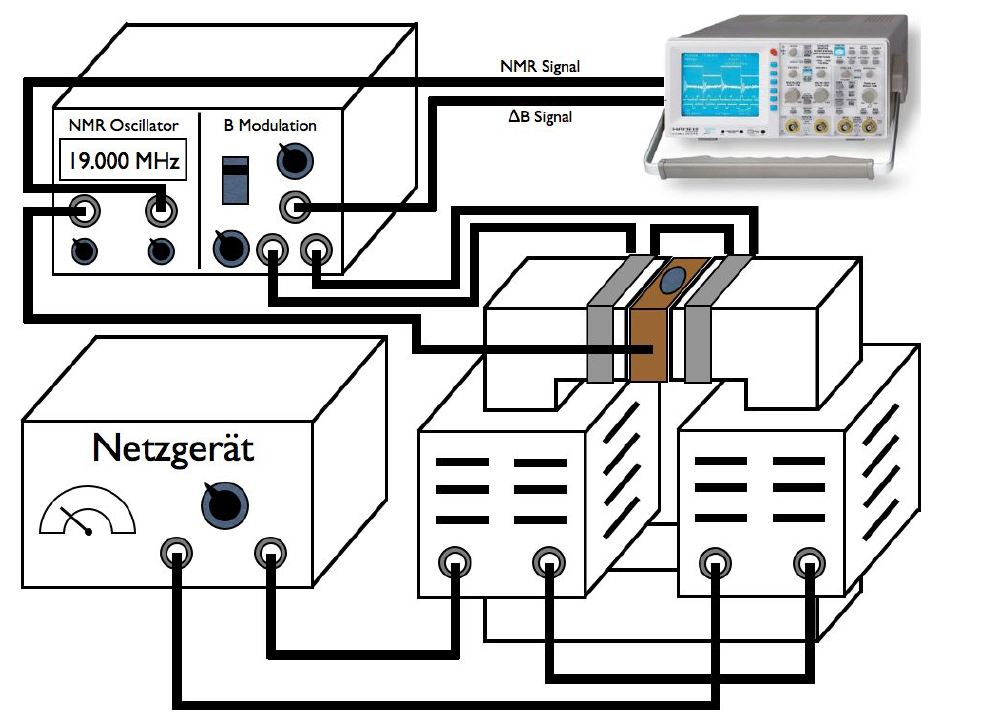
\includegraphics[scale=0.8]{Bild/Setup1}
	\centering
	\caption[Block Diagram for Setup 1]{Setup for measuring the resonance frequency with a sinus modulation.}
	\label{Exp_part1}
\end{figure}
\subsubsection{Lock-In Method}
For the second part the lock-in method is used since it is more precise duo to its lower background noise. Instead of the former absorption curve this method gives the differentiated curve. For the modulation of the magnetic field the superposition of a sinus and a sawtooth is used. Here the sawtooth is used mainly for the variance of the field while the sinus is used to create the differentiated signal since it has a similar frequency to the reference signal. The former minima of the absorption curve will now be the 'Nulldurchgang' of the signal. The moment the 'Nulldurchgang' of both measured signals overlap the correct resonance frequency is hit. Examples of both signals are shown in figure \ref{SägezahnBsp} and the setup is given in figure \ref{Exp_part2}.
\begin{figure}[ht]
	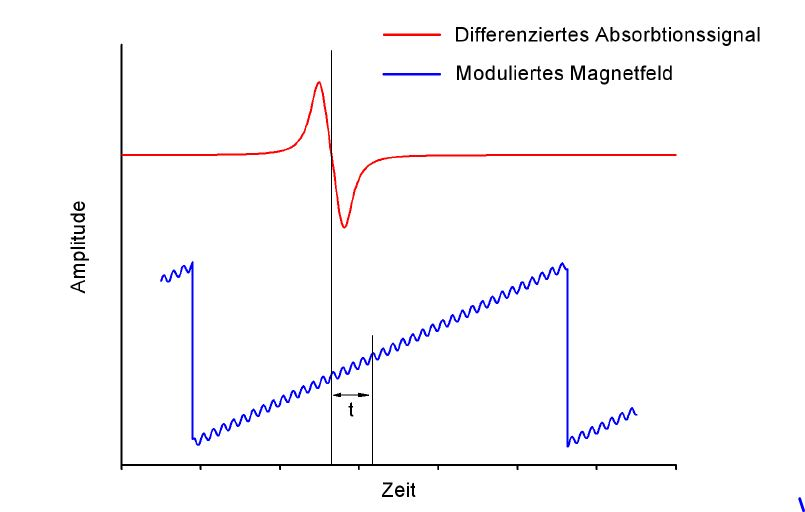
\includegraphics[scale=0.8]{Bild/BspLockIn}
	\centering
	\caption{Derived absorption signal in red. Superposition of sinus and sawtooth waves with both 'Nulldurchgängen' aligned.}
	\label{SägezahnBsp}
\end{figure}
\begin{figure}[ht]
	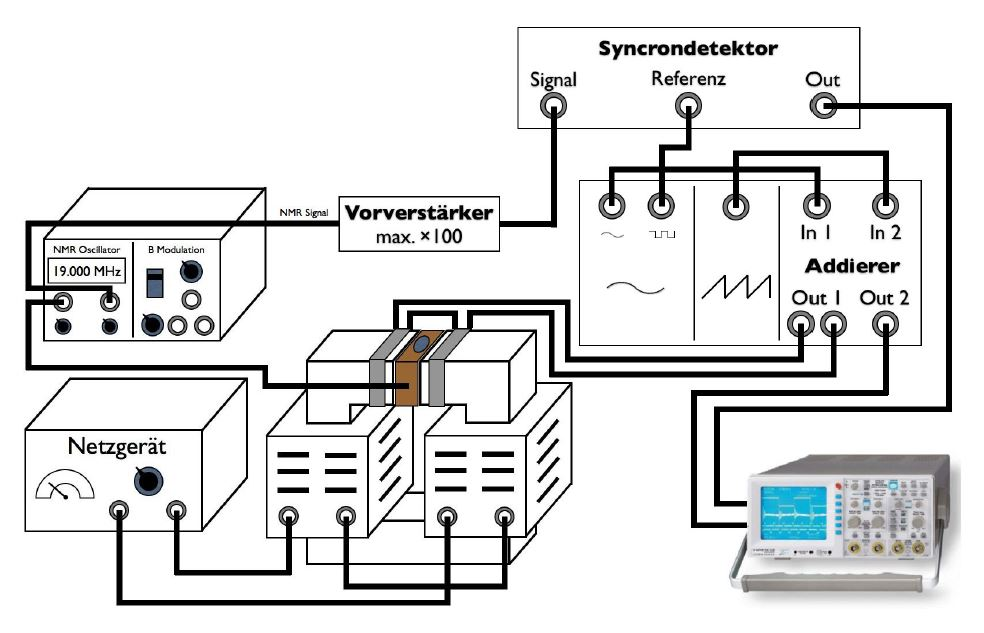
\includegraphics[scale=0.8]{Bild/Setup2}
	\centering
	\caption[Block Diagram for Setup 2]{Setup for measuring the resonance frequency with the lock-in method.}
	\label{Exp_part2}
\end{figure}


 	\section{Conduct of the Experiment}
In the beginning of the experiment it had to be checked if the magnetic field inside the setup is homogeneously distributed. For this a Hall-Sensor was used with which the field strength can be measured. Here by the sensor was slowly put into the field and depending on place the strength of the field was recorded. After conforming the uniformity of the field, a position in the middle of the homogeneous part was chosen to place the samples into.\par
With this set the experiment was set up like in figure \ref{Exp_part1} described. The measurement was started with the  Glycol sample at a depth of $2$\,cm and a constant magnetic field of $425\,$mT. With this set, the corresponding frequency of the nuclear magnetic resonance (NMR) oscillator was set by looking for the absorption peaks in the oscilloscope. After learning that it would be easier to find the rough position with a fixed frequency it became much easier to locate the peaks. The fine positioning was still done by modifying the frequency. By setting all peaks equidistant to one another the correct resonance frequency could be found. After this two underground samples were made, one without the H$_1$ sample inside the field and by setting wrong combinations of magnetic field and oscillation. The H$_1$ sample was used for all background measurements as well as for the calibration between the change in frequency and the change in position on the oscilloscope. The reason for using H$_1$ is that it has the least amount of disturbances. It is so to speak our standard candle. With the position - frequency calibration done the actually measurements were started anew. For different combinations of magnetic field and frequency with equidistant absorption lines, the CSV files were taken. After doing this for H$_1$ and Glycol the Hall-Sensor broke and another one had to be used. This one had the problem that it was strongly influenced by the temperature. This showed by the slowly decrease in measured field strength. The first value measured around the depth of $2\,$cm was noted.\par 
After finishing this way the $^{19}$F sample the Lock in Method was used to decrease the background noise. After building the setup of figure \ref{Exp_part2} a suitable resonance frequency was chosen. Here a slow shifting of the absorption peaks was noted, most likely duo to the heating of the magnets. After waiting for them to be warmed up the shifting stopped and the first measurement with the Lock in Method could be started. Here a new calibration of position and frequency was made by shifting the positions of the differentiated absorption signal.\par
Duo to some problems with the measurement of the magnetic field some measurements to the influence of the Hall-Sensor were made. One with the sawtooth voltage and one without it. With these and the voltage and ampere used to create the magnetic field, the accuracy of measurement with the new Hall-Sensor can be determined more closely.
 	\section{Analysis of the sine modeling  method}
The analysis of the sinus method consists of multiple parts: First the error threshold was computed, which will be used to determine the first absorption dip from each of the change of channels per change of frequency measurements.
Second, the change of channels per change of frequency was computed, choosing one of the dips as reference. 
Third, the actual resonance frequency for each measurement was computed with the relation of the second step of this part of the analysis.
Fourth, the combination of the measured magnetic fields and computed frequencies was used to compute the magnetic momentum of the proton in $^{19}$F and the gyromagnetic ratio of the proton in glycol and hydrogen.
\subsection{Error thresholds}
%  Although two different pure background measurements were recorded, they ended up replaced by the noise recorded during the measurements for the change of channel per change of frequency.
For the error thresholds, one has to take a closer look at the recorded data. The .csv files obtained during the experiment contain the maxima and minima of the curves seen on the oscilloscope. To get a limit which is useful to discriminate the data multiple preparatory steps were necessary: First the absolute values of the differences from two neighbouring background data points were computed and projected to the y axis. A Gaussian curve was fitted to this projection. The maximum of the fitted curve, subtracted from to the mean of the background data used for the projection was the lower error threshold.\par 
In comparison to the out sample or in sample of frequency background, the background during the actual measurement is the most representative, because it was obtained during the exact same conditions as the signal data.
After taking an initial look at the measurements used for the frequency difference per channel difference (as seen in fig. \ref{all_dx}), it was decided that a sufficient amount of background data points can be obtained from these measurements. 
\begin{figure}[h]
	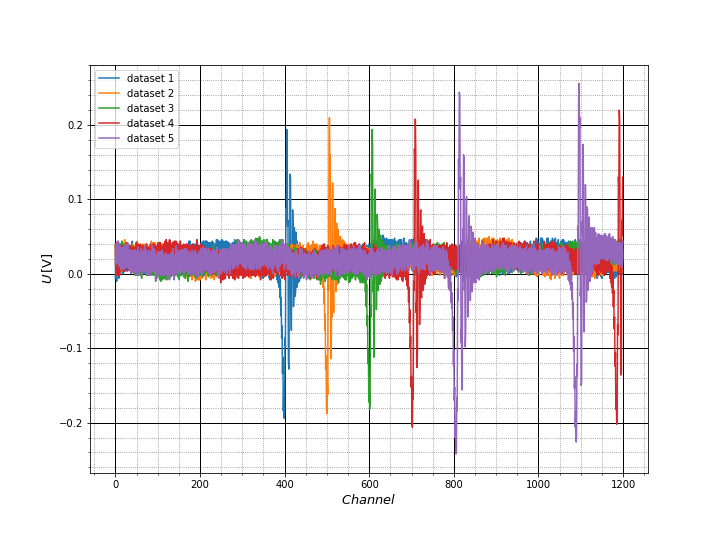
\includegraphics[scale=0.5]{Bild/all_dx.png}
	\centering
	\caption[Plot of all data used for the discriminator determination]{Plot of the measured voltage against the channel of the data points from all five measurements used for the difference in frequency per difference in channel.}
	\label{all_dx}
\end{figure}

After examining the first absorption peak of the first dataset, the parameter to coarsely seperate the background from the absorbtion signals was determined to be $-0.03\,$V. Both can be seen in fig. \ref{absorbtionpeak}. All values up to the tenth value underneath this threshold are considered as background signal.\par
\begin{figure}[h]
	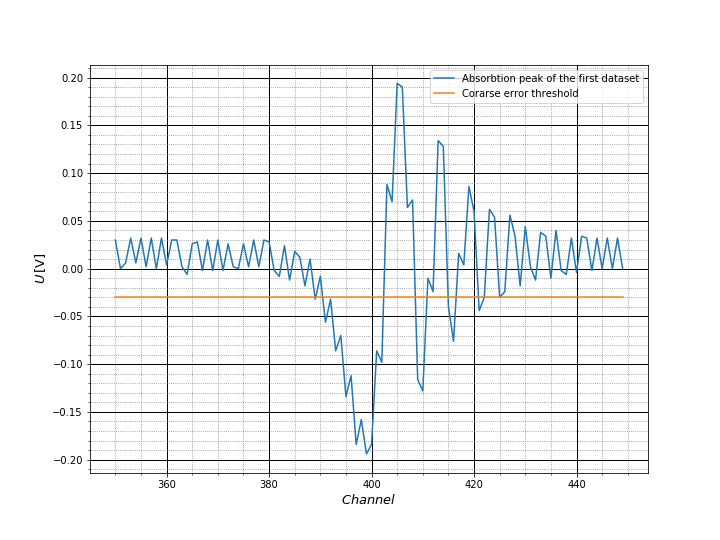
\includegraphics[scale=0.5]{Bild/peak_first_single.png}
	\centering
	\caption[Plot of an absorption peak]{Plot of the measured voltage against the channel of the absorption peak of the first measurement taken for the frequency change channel change ration measurement series. Also seen is the coarse error threshold of $-0.03\,$V.}
	\label{absorbtionpeak}
\end{figure}

All of these values can be seen in fig. \ref{all_err}. Now, the absolute difference between two neighbouring points was computed, which can be seen in fig. \ref{err_abs}. It is clearly visible, that all the data points in fig. \ref{all_err} and absolute differences in fig. \ref{err_abs} come in discrete levels. The reason behind this is the limited resolution of the analogue digital converter in the oscilloscope, which represents the values as binary numbers of a certain length, allowing only discrete voltage levels to be displayed. \par
These discrete levels result in zeros in the projection of the values to the y axis, which were not considered for the fit of the Gaussian curve. 

 	\section{Analysis of the Lockin Method}
For the analysis the 'Nulldurchgang' of both the Lock-In and the sawtooth signal needs to be calculated. First of all the slopes of the measured sawtooth were fitted with a linear fit of the form $f(x)=m\cdot x+b$. For the fit \verb|curve_fit| of the python package \verb|scipy.optimize| \cite{SciPy_Opti} was used. With these parameters the 'Nulldurchgang' for each measurement can be calculated. To do so equation \ref{Nulldurchgang1} was used, with $d_s$ being the position were the curve crosses zero. The error $\sigma_{d_s}$ is calculated using Gaussian error propagation.
\begin{equation}
	d_S=-\frac{b}{m}
	\label{Nulldurchgang1}
\end{equation}
\begin{equation}
	\sigma_{d_S}=\sqrt{(\frac{\sigma_{b}}{m})^2+(\frac{b}{m^2}\sigma_{m})^2}
\end{equation}
The parameters and 'Nulldurchgang' are documented in table \ref{SägezahnParameter}. The figures of the measured signals as well as the corresponding fits can be seen for the data of the CSV file \verb|lockin_9| in figure \ref{Example}. The other ones can be found in the appendix in figure \ref{Lock2} to \ref{Lock7}.\par
\begin{figure}[ht]
	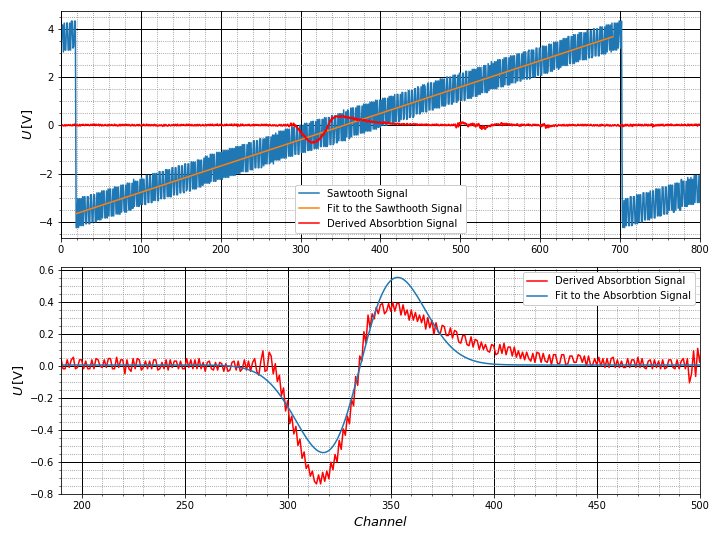
\includegraphics[scale=0.5]{Bild/LockIn8.png}
	\centering
	\caption[Plots and Fits of Lock-In Method 1]{\small The upper figure shows the data of the sawtooth in blue with the corresponding fit in orange. The absorption signal is in red. The lower one shows the part of the absorption signal which is of interest with the fit in blue.}
	\label{Example}
\end{figure}
For the high frequency signal (HF) of the NMR Oscillator the derivative of an inverse Gaussian curve was fitted. The form can be seen in eq.\ref{gaussian_ab}.
\begin{equation}
	f(x)=\frac{a(x-d_{A})e^{-\frac{(x-d_{A})^2}{2c^2}}}{c^2}+h
	\label{gaussian_ab}
\end{equation}
As can be seen in figure \ref{Example} the fits aren't very similar to the measured data. The main problem is the asymmetry of the amplitudes which are different for the data but are expected to be similar in eq.\ref{gaussian_ab}. The reason for this is very likely the Lock-In method as well as relaxation processes duo to which the expected Gaussian derivative is not a perfect match. The reason this fit was still used is that the needed parameter $d_{A}$ which gives the 'Nullstelle' isn't affected to much. This can also be seen in table \ref{GaussianTable} since here the errors on the listed parameters $d_A$, which give the needed 'Nullstellen' position, aren't to high.\par
With those two positions of the sawtooth as well as the absorption signal the distance $\Delta d$ between those can be calculated and depicted together with the corresponding frequency of the NMR Oscillator. The error for this gab $\sigma_{\Delta d}$ is calculated using eq.\ref{Gab}. 
\begin{equation}
	\sigma_{\Delta d}=\sqrt{(d_A\sigma_{dS})^2+(d_S\sigma_{dA})^2}
	\label{Gab}
\end{equation}
The data points were than fitted with the linear form $f(x)=m_2\cdot x+b_2$. The difference to the sawtooth fit is, that the error $\sigma_{\Delta d}$ was used for this fit. Since \verb|curve_fit| only takes errors of the y-axis, the errors for the frequency weren't used since they aren't as dominant for the calculation. The data points and the fit are shown in figure \ref{Nullstellenfit}. The data points coloured in green were excluded from the fit calculation. The reason for this is warming up of the magnets and the long time between the measurement of these two points and the others. This caused a slow shifting in the magnetic field and with that a shift in the resonance frequency.\par
\begin{figure}[h]
	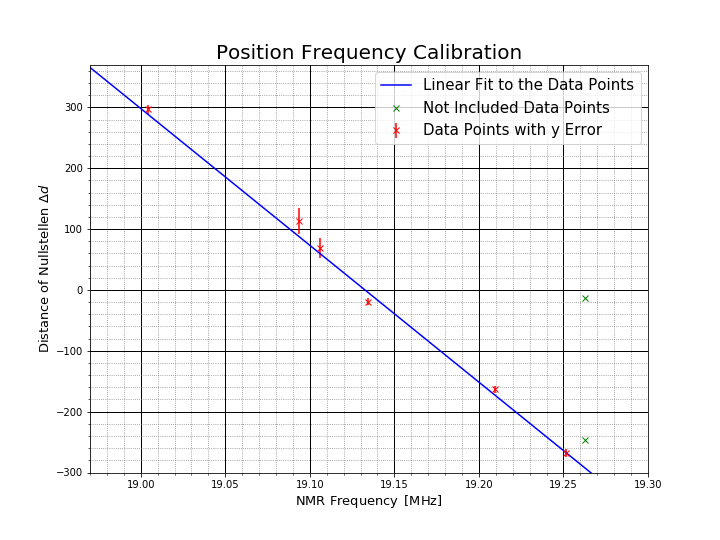
\includegraphics[scale=0.5]{Bild/Eichung.png}
	\centering
	\caption[Distance of 'Nullstellen' to Frequency Plot]{Plot of frequency against the distance $\Delta d$. The green data points were excluded from the fit calculation. The fit itself is calculated with the errors $\sigma_{\Delta d}$.}
	\label{Nullstellenfit}
\end{figure}
With the help of this fit the resonance frequency at which both 'Nullstellen' align can be found, since here the value for $\Delta d$ is zero. Using equation \ref{Nullstelle2} the frequency and its error were calculated.
\begin{equation}
f_{LockIn}=-\frac{b_2}{m_2}
\label{Nullstelle2}
\end{equation}
\begin{equation}
\sigma_{d_S}=\sqrt{(\frac{\sigma_{b}}{m})^2+(\frac{b}{m^2}\sigma_{m})^2}
\end{equation}
The resonance frequency for the Lock-In method we get using this calculation is:$$f_{LockIn}=(19.1\pm0.6)\,\text{MHz}$$
The corresponding magnetic field is calculated using the mean of the measured magnetic fields while the error is calculated using equation \ref{error Mean}.
\begin{equation}
	\sigma_x=\sqrt{\frac{1}{1-n}\sum_{n}^{i=1}(x_i-\bar{x})^2}
	\label{error Mean}
\end{equation}
Here the first 3 measured B-fields were excluded. The reason for the first two is similar to the excluded data points in fig.\ref{Nullstellenfit}. The third one was excluded duo to its huge difference to the other values. The reason the difference is either that the sawtooth wasn't turned off, or the hall sensor was to long inside the magnetic field which increased the temperature. The problems with the Hall sensor are discussed in the conclusion. With that the magnetic field is at:
$$B_{LockIn} = (463.0\pm0.7)\,\text{mT}$$
\subsection{Hall Sensor}
For the measurement of the homogeneity of the field the data points were plotted in figure \ref{Homogen}. It can be seen clearly that after a depth of $7$\,mm inside the field no change is noticeable so our field is uniform at this point.
\begin{figure}[ht]
	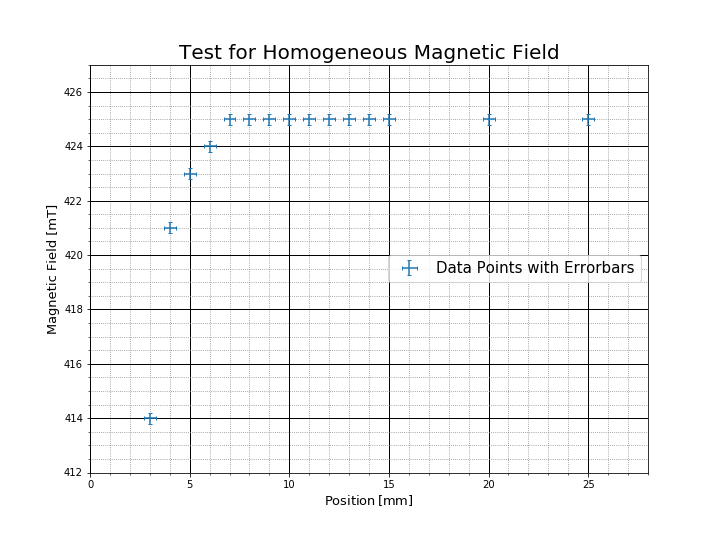
\includegraphics[scale=0.5]{Bild/Hallsonde}
	\centering
	\caption[Uniformity of the Magnetic Field]{The strength of the magnetic field depending on the depth inside the field.}
	\label{Homogen}
\end{figure}\\
Since the first Hall sensor was destroyed during the experiment another one had to be used. This one showed a change in the magnetic field depending on the time it was inside the field. To increase the accuracy of the experiment this change was measured once with the sawtooth and once without it. These two can be seen in figure \ref{Hallsonde1} and \ref{Hallsonde2}.
\begin{figure}[ht]
	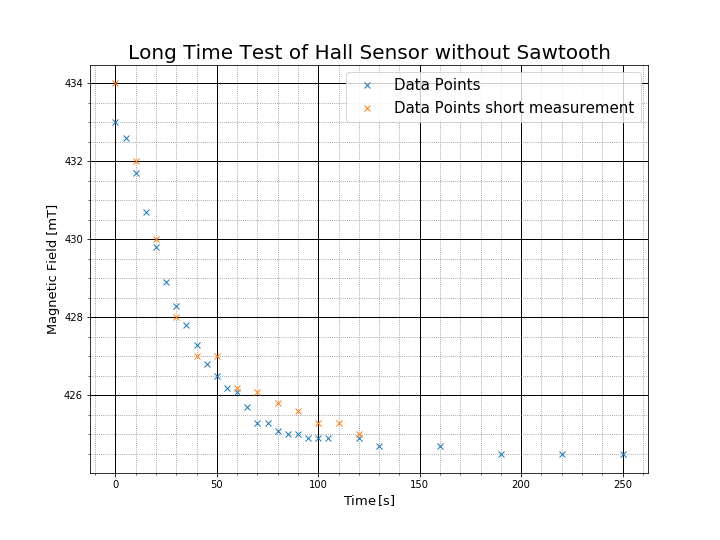
\includegraphics[scale=0.5]{Bild/Hallsonde1}
	\centering
	\caption[Hall Sensor without Sawtooth]{Measurement of the magnetic field depending of the time inside the field with the sawtooth shaped signal. The errors for the data points were to small to make them clearly visible.}
	\label{Hallsonde1}
\end{figure}
\begin{figure}[ht]
	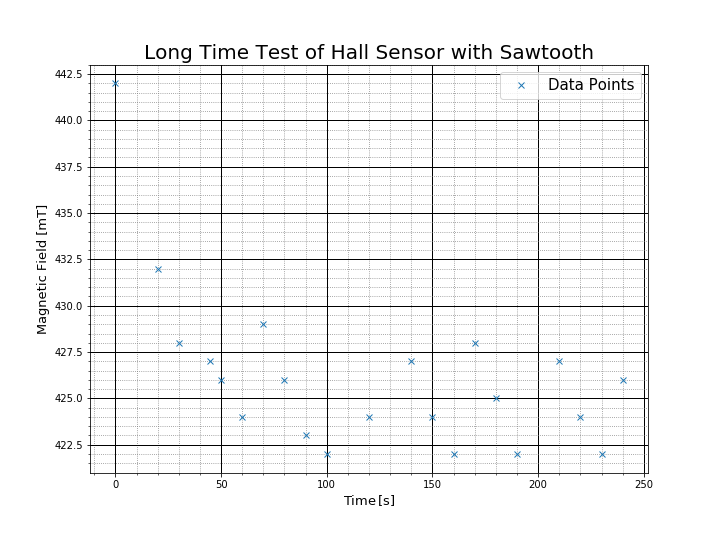
\includegraphics[scale=0.5]{Bild/Hallsonde2}
	\centering
	\caption[Hall Sensor with Sawtooth]{Measurement of the magnetic field depending of the time inside the field without the sawtooth shaped signal. Here two measurements were made one in orange the other one in blue. The errors for the data points were to small to make them clearly visible.}
	\label{Hallsonde2}
\end{figure}
It is clearly visible that time has an impact on the measurement. In fig.\ref{Hallsonde1} we the that for once the change from the sawtooth which slowly decreases the magnetic field and than increases it suddenly. In fig.\ref{Hallsonde2} the saturation of after a certain time is seen. It is very likely that the temperature inside point of measurement changes the properties of the Hall sensor. With that it is not clear which is the correct magnetic field. The one at the saturation or the beginning when the sensor is close the room temperature. Inside the manual of the electro magnets a hysteresis curve was found giving the magnetic field depending on the amperage.\cite{Electromagnet} Since the amperage during the measurement was at $3.41$\,A the magnetic field strength should be around $415$,mT. This value is not very precise since the curve could have changed over time but it clearly shows, that the saturation value is more precise. Since the upper one was used for the measurements, a large systematic error has to be expected for all measurements taken with the new Hall sensor.
 	\section{Zusammenfassung}
Wenn man die gemessenen Werte mit denen des Literatur Wertes von $119\,$ns mit der Formel \ref{Vergleich} vergleicht erhält man die in Tabelle \ref{VglTable} beschriebenen Werte. \\
\begin{table}
	\begin{Dtabular}[1.1]{|c|c|c|}
		\hline
		Messreihe&Lebensdauer $\tau$[ns]&Vergleichswert\\
		\hline
		Abkühlen 1 bei $0^\circ$&$(1.224\pm0.022)$&\\
		\hline
		Abkühlen 1 bei $90^\circ$&&\\
		\hline
		Aufwärmen bei $0^\circ$&&\\
		\hline
		Abkühlen 2 bei $0^\circ$&&\\
		\hline
		Abkühlen 2 bei $90^\circ$&&\\
		\hline
	\end{Dtabular}
\end{table}
Man erkennt schnell, dass alle gemessenen Werte bis auf die Aufwärmmessung mit dem Literaturwert kompatibel sind. Die große Diskrepanz kann man dadurch erklären, dass für die Messung während des Aufwärmvorgangs nicht gewartet wurde bis die Temperatur des Thermometers mit der der Probe angeglichen hat. Dadurch ziehen wir einen großen systematischen Fehler mit welcher die Unverträglichkeit erklären könnte. \par Ein weiteres Problem ist sicher die geringe Anzahl an Messpunkten die wir in allen Messreihen hatten, wodurch sich natürlich unsere Messreihe verschlechtert. 
 	
 	
 	
 	
 	
 	\section{List of tables}
 	\listoftables
 	\section{List of Figures}
 	\listoffigures
 	\section{Bibliograpy}
 		\bibliographystyle{plain}
 		\bibliography{Quellen}
 		\addcontentsline{toc}{section}{Literatur}
 	\section{Appendix}
 	\begin{figure}
	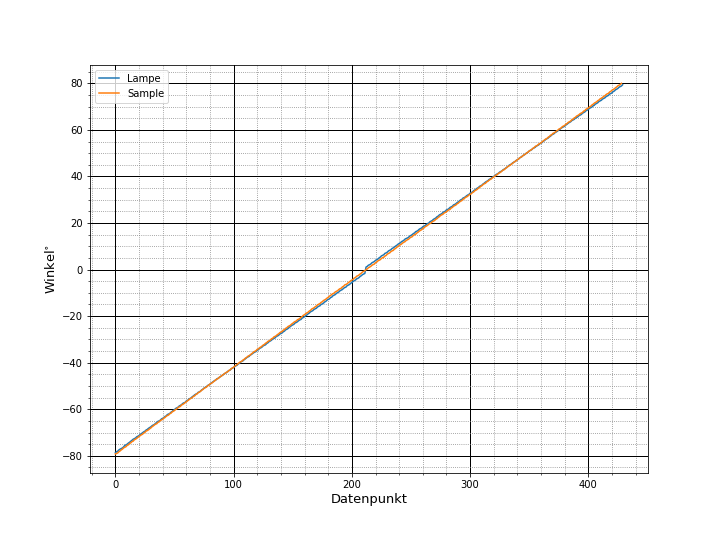
\includegraphics[scale=0.5]{Bilder/anhang/korrektur_channels_2}
	\centering
	\caption[Korrigierter Lampendatensatz 2. Silizium messung]{\small Auftragung der gemessenen Winkel für die Lampenmessung und erste Silizium Messung nach der Korrektur. Beide stimmen in den relevanten Bereichen bei ca. $30^{\circ}-40^{\circ}$ weitgehend überein.}
\end{figure}
\begin{figure}
	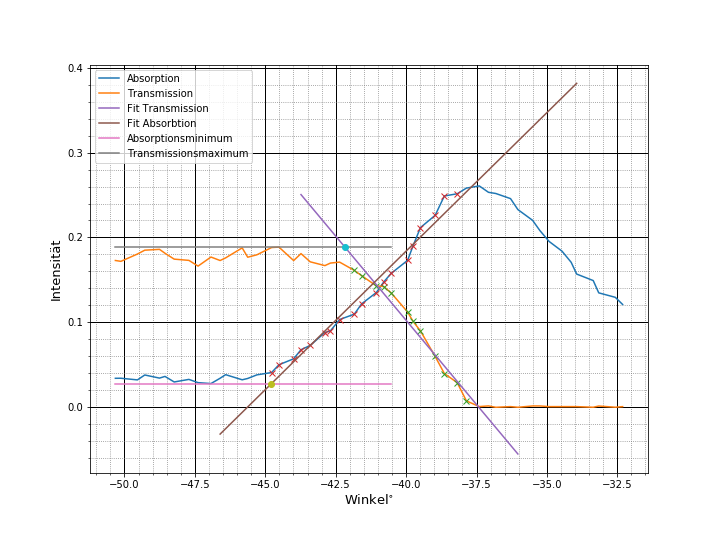
\includegraphics[scale=0.5]{Bilder/anhang/si_2_l}
	\centering
	\caption[Geraden Anpassungen 2. Silizium Messung links]{\small Auftragung von Intensität der normalisierten Datenreihen gegen die  Winkel in der Nähe der Stelle Gleichwahrscheinlicher Absorption und Transmission bei Winkeln kleiner als $0^\circ$. Es sind zusätzlich die angepassten Geraden zur Absorption und Transmission eingezeichnet. Die Horizontalen wurden durch die Maxima der dahinterliegenden Datenpunkte bestimmt. Die Schnittpunkte der Geraden mit ihren jeweiligen Horizontalen sind auch eingezeichnet.}
\end{figure}
\begin{figure}
	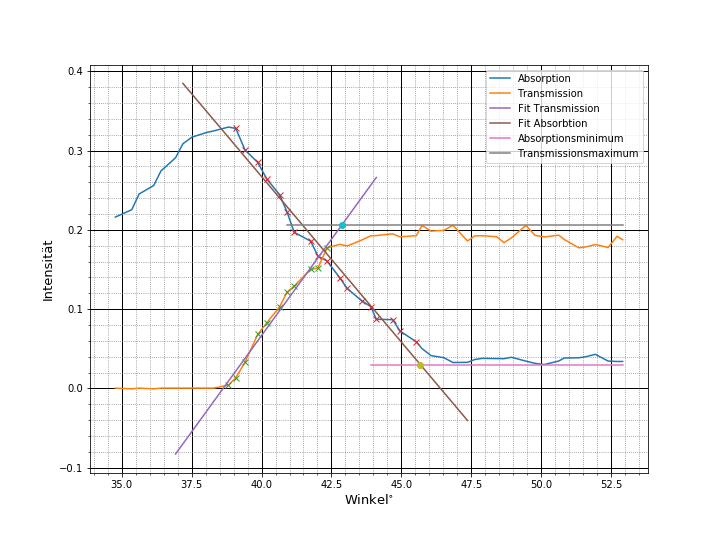
\includegraphics[scale=0.5]{Bilder/anhang/si_2_r}
	\centering
	\caption[Geraden Anpassungen 2. Silizium Messung rechts]{\small Auftragung von Intensität der normalisierten Datenreihen gegen die  Winkel der zweiten Silizium Messung in der Nähe der Stelle Gleichwahrscheinlicher Absorption und Transmission bei Winkeln größer als $0^\circ$. Es sind zusätzlich die angepassten Geraden zur Absorption und Transmission eingezeichnet. Die Horizontalen wurden durch die Maxima der dahinterliegenden Datenpunkte bestimmt. Die Schnittpunkte der Geraden mit ihren jeweiligen Horizontalen sind auch eingezeichnet.}
	\label{si_2_r}
\end{figure}
\begin{figure}
	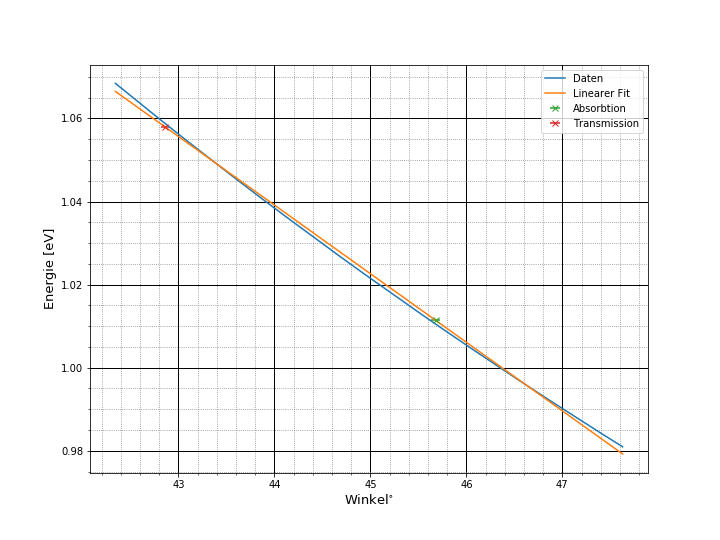
\includegraphics[scale=0.5]{Bilder/anhang/si_2_l_energie}
	\centering
	\caption[Energiebestimmung 2. Si Messung links]{\small Auftragung der Energie gegen den Winkel der zweiten Silizium Messung. Die angepasste Gerade und die beiden Schnittpunkte sind auch eingetragen.}
\end{figure}
\begin{figure}
	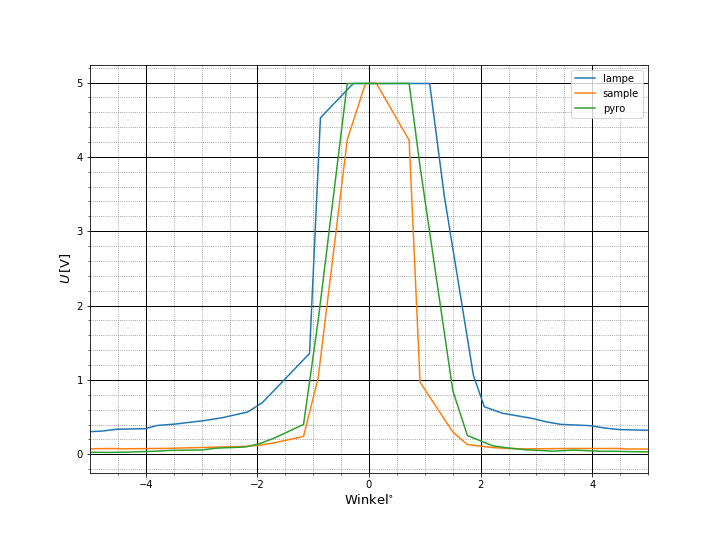
\includegraphics[scale=0.5]{Bilder/anhang/winkelkorrektur_vorher}
	\centering
	\caption[Mittelpunkt der 2. Si Messung vor Winkelkorrektur]{\small Auftragung der Intensität gegen den Winkel der zweiten Silizium Messung in der Nähe von $0^\circ$ vor der Korrektur.}
\end{figure}
\begin{figure}
	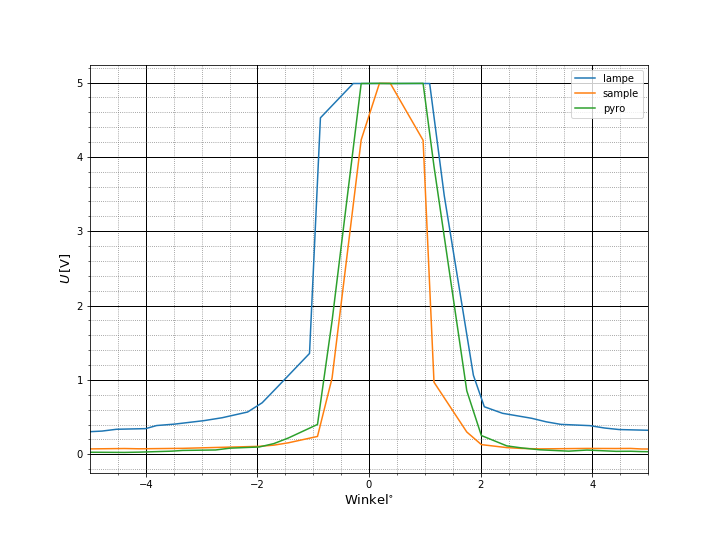
\includegraphics[scale=0.5]{Bilder/anhang/winkelkorrektur_nachher}
	\centering
	\caption[Mittelpunkt der 2. Si Messung vor Winkelkorrektur]{\small Auftragung der Intensität gegen den Winkel der zweiten Silizium Messung in der Nähe von $0^\circ$ nach der Korrektur.}
\end{figure}
\begin{figure}
	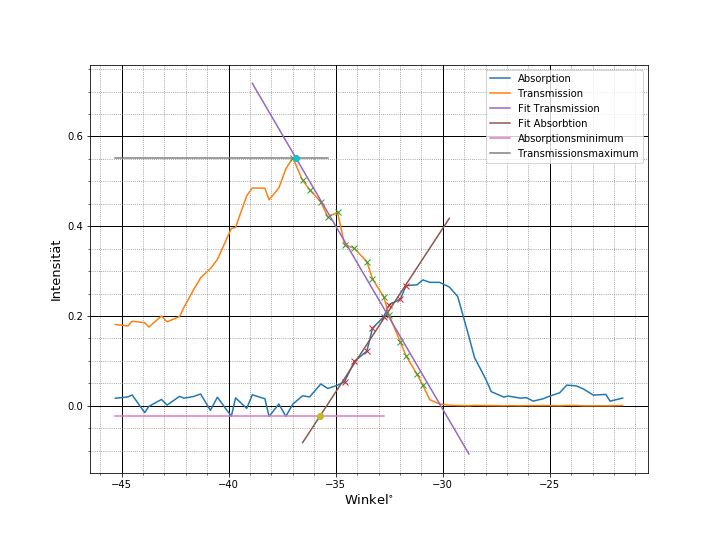
\includegraphics[scale=0.5]{Bilder/anhang/ge_r}
	\caption[Geraden Anpassungen Germanium Messung links]{\small Auftragung von Intensität der normalisierten Datenreihen von Germanium gegen die  Winkel in der Nähe der Stelle Gleichwahrscheinlicher Absorption und Transmission bei Winkeln größer als $0^\circ$. Es sind zusätzlich die angepassten Geraden zur Absorption und Transmission eingezeichnet. Die Horizontalen wurden durch die Maxima der dahinterliegenden Datenpunkte bestimmt. Die Schnittpunkte der Geraden mit ihren jeweiligen Horizontalen sind auch eingezeichnet.}
\end{figure}
\begin{figure}
	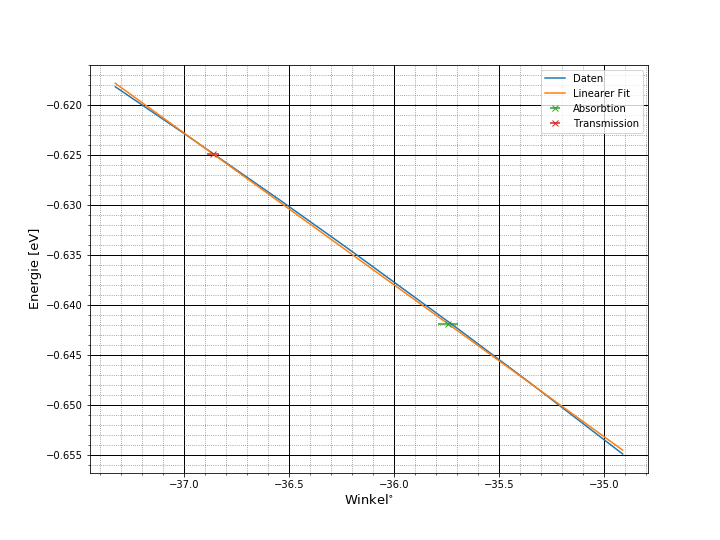
\includegraphics[scale=0.5]{Bilder/anhang/ge_l_energie}
	\centering
	\caption[Energiebestimmung Ge Messung links]{\small Auftragung der Energie gegen den Winkel der Germanium Messung. Die angepasste Gerade und die beiden Schnittpunkte sind auch eingetragen.}
\end{figure}


\begin{figure}
	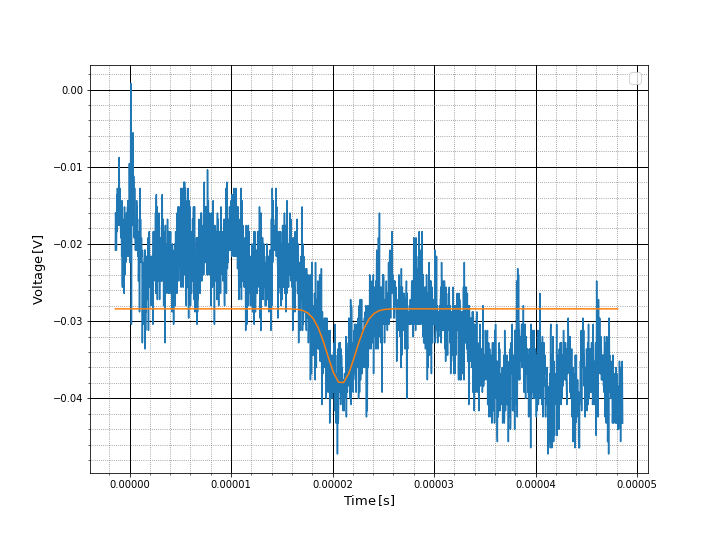
\includegraphics[scale=0.5]{Bild/S1}
	\centering
	\caption[Gaußfit an Messung bei Konst. Spannung 1]{Gaußfit an die Messungen der Elektronenwolken bei einer Spannung von $48\,$V und einem Abstand zwischen Nadel und Lase von $10.6$\,mm.}
\end{figure}
\begin{figure}
	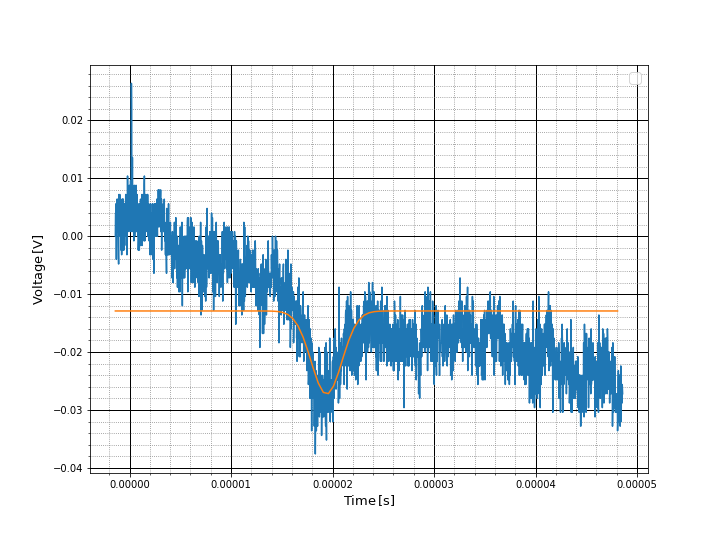
\includegraphics[scale=0.5]{Bild/S2}
	\centering
	\caption[Gaußfit an Messung bei Konst. Spannung 2]{Gaußfit an die Messungen der Elektronenwolken bei einer Spannung von $48\,$V und einem Abstand zwischen Nadel und Lase von $9.6$\,mm.}
\end{figure}
\begin{figure}
	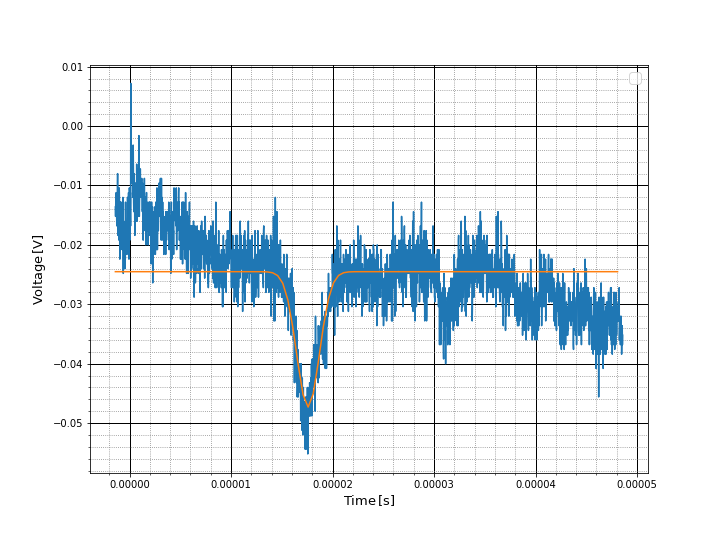
\includegraphics[scale=0.5]{Bild/S3}
	\centering
	\caption[Gaußfit an Messung bei Konst. Spannung 3]{Gaußfit an die Messungen der Elektronenwolken bei  einer Spannung von $48\,$V und einem Abstand zwischen Nadel und Lase von $8.6$\,mm.}
\end{figure}
\begin{figure}
	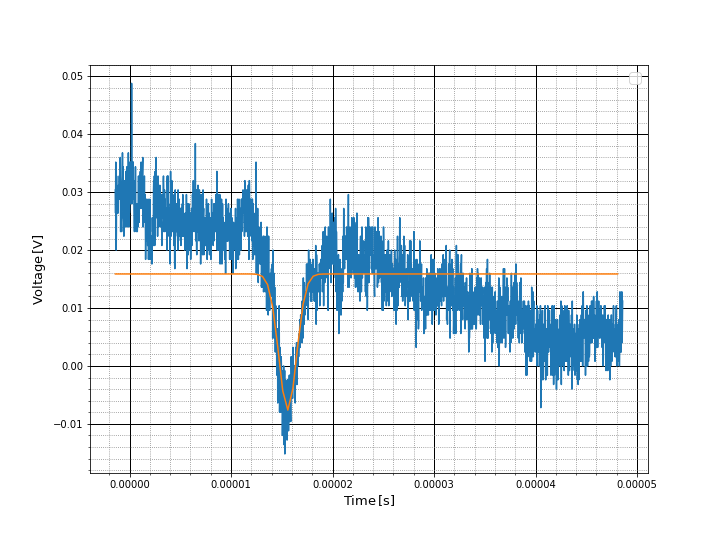
\includegraphics[scale=0.5]{Bild/S4}
	\centering
	\caption[Gaußfit an Messung bei Konst. Spannung 4]{Gaußfit an die Messungen der Elektronenwolken bei  einer Spannung von $48\,$V und einem Abstand zwischen Nadel und Lase von $7.6$\,mm.}
\end{figure}
\begin{figure}
	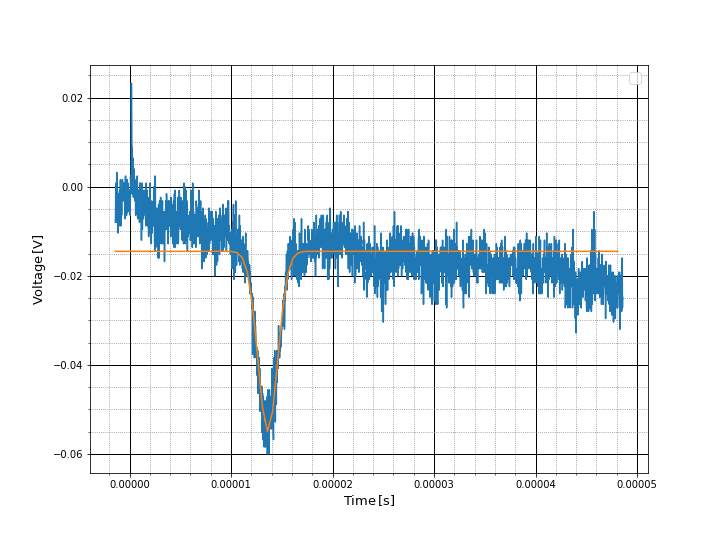
\includegraphics[scale=0.5]{Bild/S5}
	\centering
	\caption[Gaußfit an Messung bei Konst. Spannung 5]{Gaußfit an die Messungen der Elektronenwolken bei einer Spannung von $48\,$V und einem Abstand zwischen Nadel und Lase von $6.6$\,mm.}
\end{figure}
\begin{figure}
	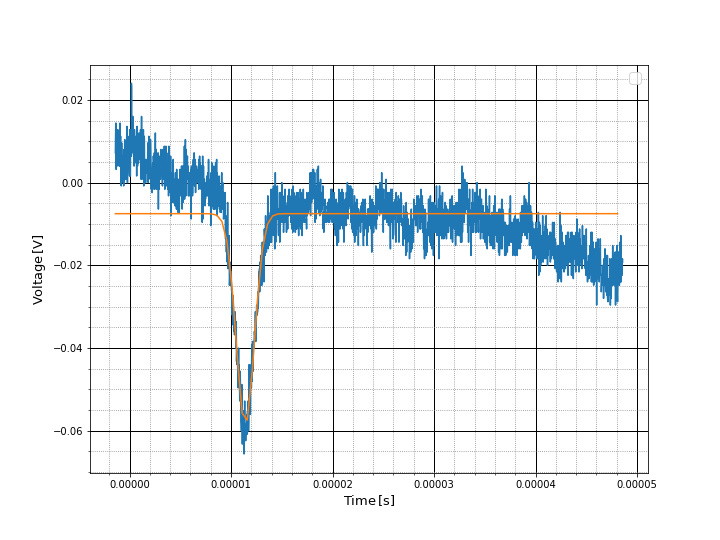
\includegraphics[scale=0.5]{Bild/S6}
	\centering
	\caption[Gaußfit an Messung bei Konst. Spannung 6]{Gaußfit an die Messungen der Elektronenwolken bei einer Spannung von $48\,$V und einem Abstand zwischen Nadel und Lase von $5.6$\,mm.}
\end{figure}
\begin{figure}
	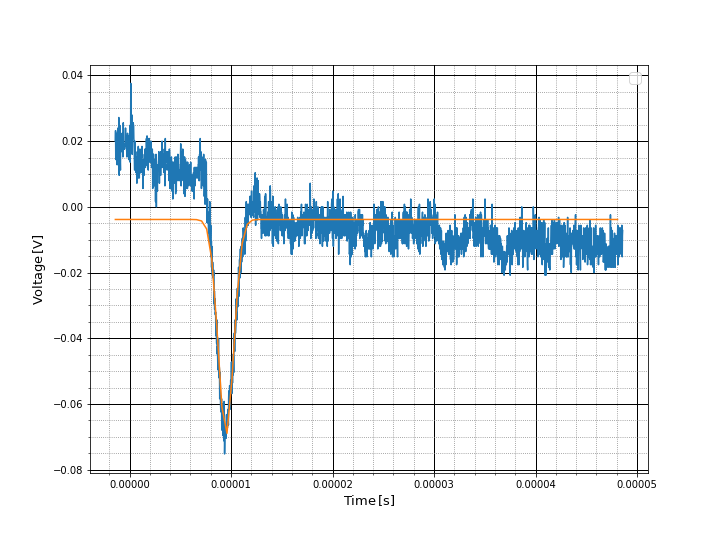
\includegraphics[scale=0.5]{Bild/S7}
	\centering
	\caption[Gaußfit an Messung bei Konst. Spannung 7]{Gaußfit an die Messungen der Elektronenwolken bei einer Spannung von $48\,$V und einem Abstand zwischen Nadel und Lase von $4.6$\,mm.}
\end{figure}
\begin{figure}
	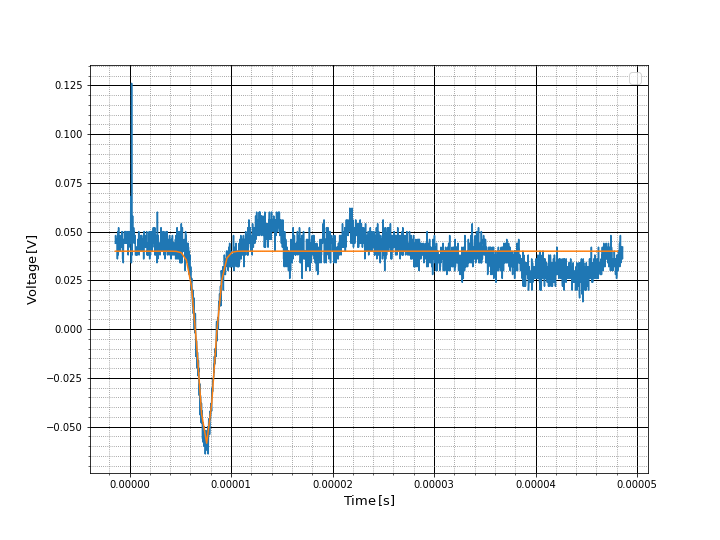
\includegraphics[scale=0.5]{Bild/S8}
	\centering
	\caption[Gaußfit an Messung bei Konst. Spannung 8]{Gaußfit an die Messungen der Elektronenwolken bei einer Spannung von $48\,$V und einem Abstand zwischen Nadel und Lase von $3.6$\,mm.}
\end{figure}

%Andere Messreihe

\begin{figure}
	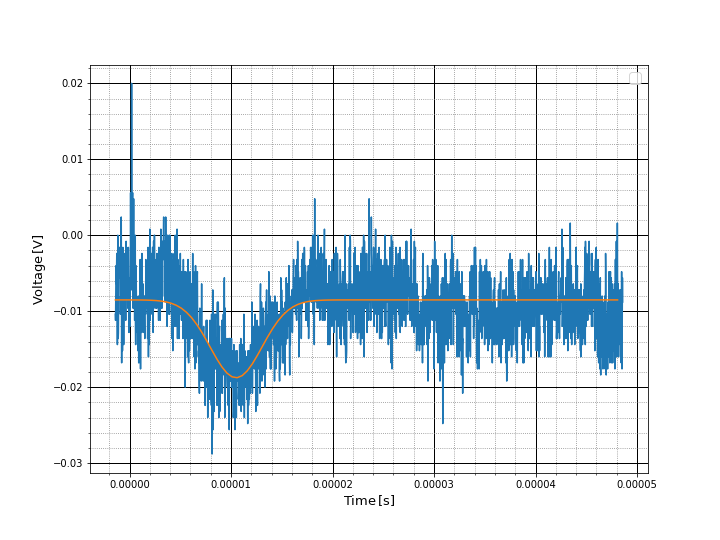
\includegraphics[scale=0.5]{Bild/A1}
	\centering
	\caption[Gaußfit an Messung bei Konst. Abstand]{Gaußfit an die Messungen der Elektronenwolken bei Konstantem Abstand von $3.6$\,mm und einer Spannung von $-13.2$\,V}
\end{figure}
\begin{figure}
	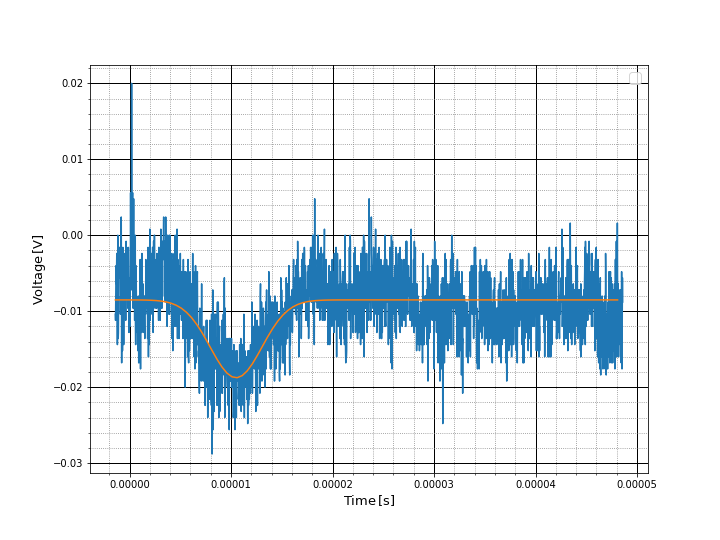
\includegraphics[scale=0.5]{Bild/A1}
	\centering
	\caption[Gaußfit an Messung bei Konst. Abstand]{Gaußfit an die Messungen der Elektronenwolken bei Konstantem Abstand von $3.6$\,mm und einer Spannung von $-15.2$\,V}
\end{figure}
\begin{figure}
	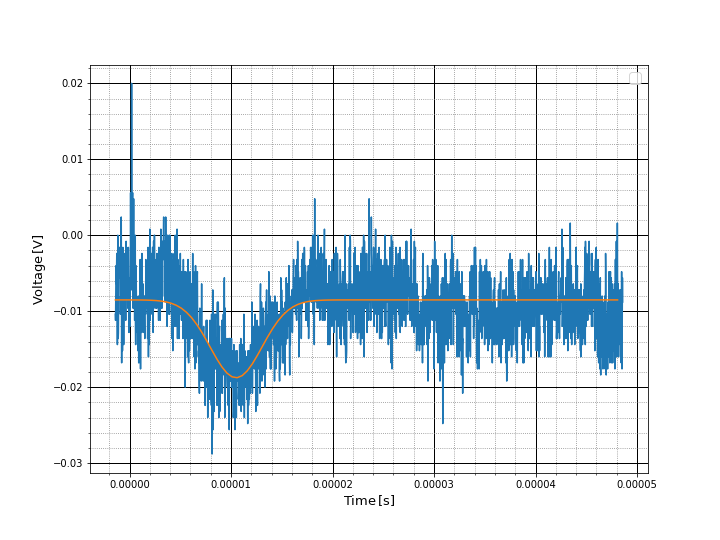
\includegraphics[scale=0.5]{Bild/A1}
	\centering
	\caption[Gaußfit an Messung bei Konst. Abstand]{Gaußfit an die Messungen der Elektronenwolken bei Konstantem Abstand von $3.6$\,mm und einer Spannung von $-18.4$\,V}
\end{figure}
\begin{figure}
	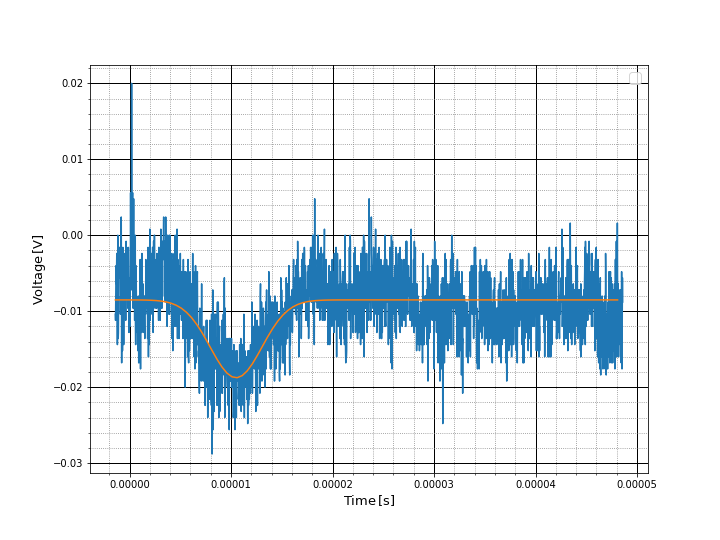
\includegraphics[scale=0.5]{Bild/A1}
	\centering
	\caption[Gaußfit an Messung bei Konst. Abstand]{Gaußfit an die Messungen der Elektronenwolken bei Konstantem Abstand von $3.6$\,mm und einer Spannung von $-20.4$\,V}
\end{figure}
\begin{figure}
	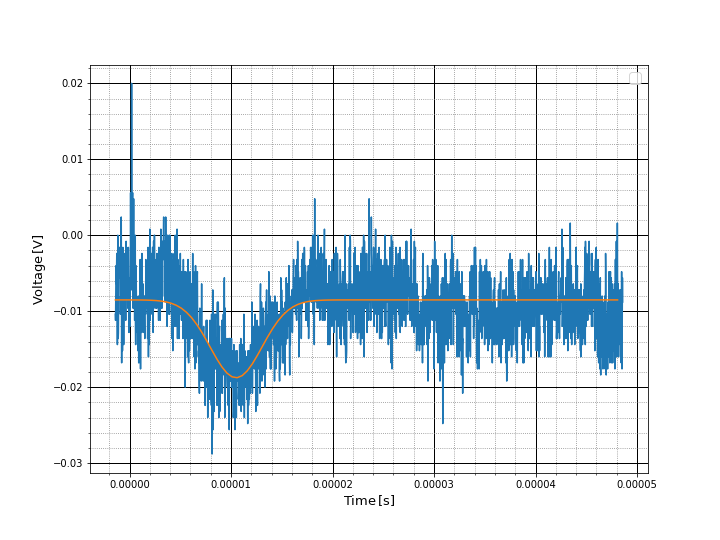
\includegraphics[scale=0.5]{Bild/A1}
	\centering
	\caption[Gaußfit an Messung bei Konst. Abstand]{Gaußfit an die Messungen der Elektronenwolken bei Konstantem Abstand von $3.6$\,mm und einer Spannung von $-22.4$\,V}
\end{figure}
\begin{figure}
	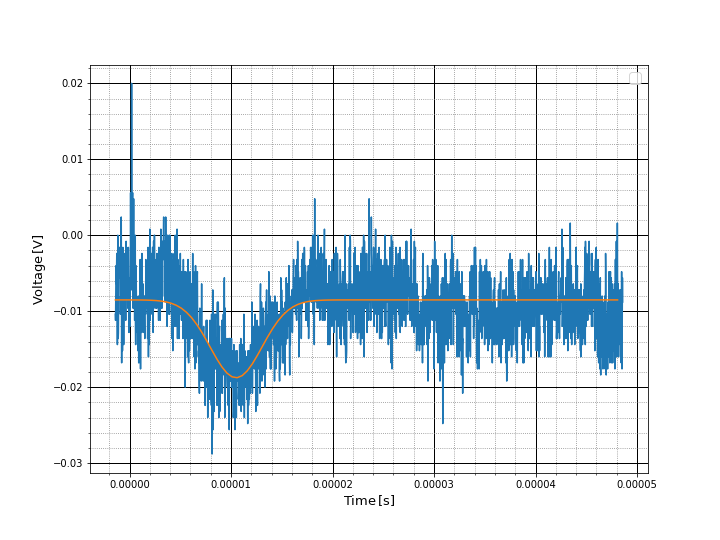
\includegraphics[scale=0.5]{Bild/A1}
	\centering
	\caption[Gaußfit an Messung bei Konst. Abstand]{Gaußfit an die Messungen der Elektronenwolken bei Konstantem Abstand von $3.6$\,mm und einer Spannung von $-24.4$\,V}
\end{figure}
\begin{figure}
	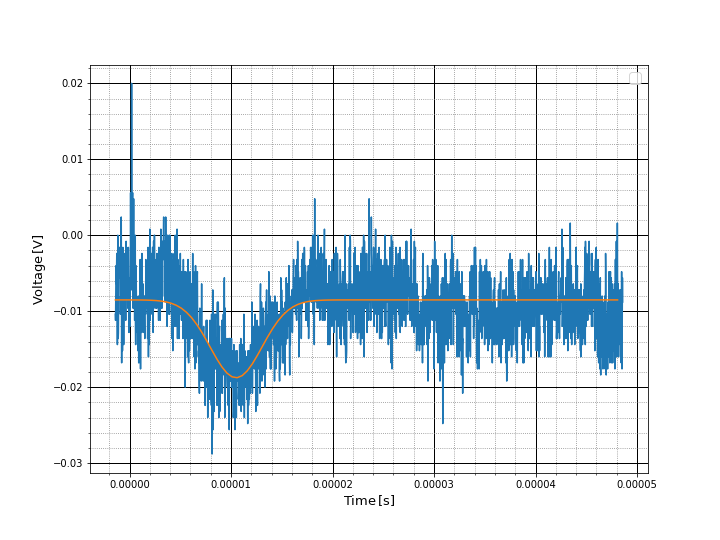
\includegraphics[scale=0.5]{Bild/A1}
	\centering
	\caption[Gaußfit an Messung bei Konst. Abstand]{Gaußfit an die Messungen der Elektronenwolken bei Konstantem Abstand von $3.6$\,mm und einer Spannung von $-28.0$\,V}
\end{figure}
\begin{figure}
	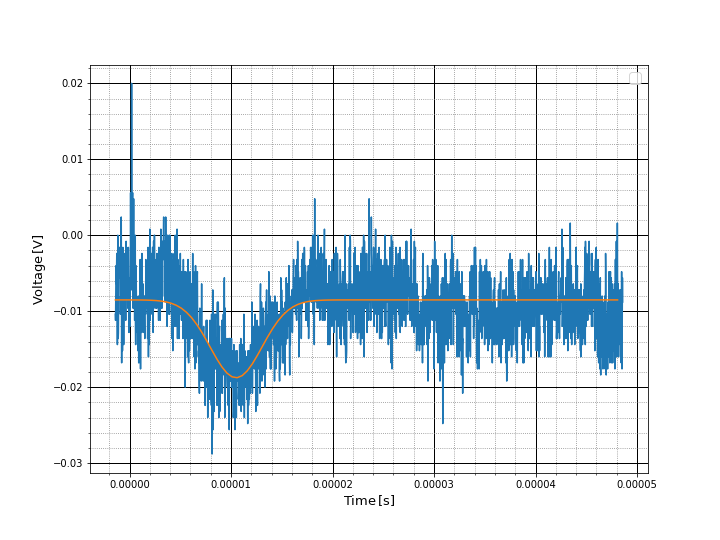
\includegraphics[scale=0.5]{Bild/A1}
	\centering
	\caption[Gaußfit an Messung bei Konst. Abstand]{Gaußfit an die Messungen der Elektronenwolken bei Konstantem Abstand von $3.6$\,mm und einer Spannung von $-32.0$\,V}
\end{figure}
\begin{figure}
	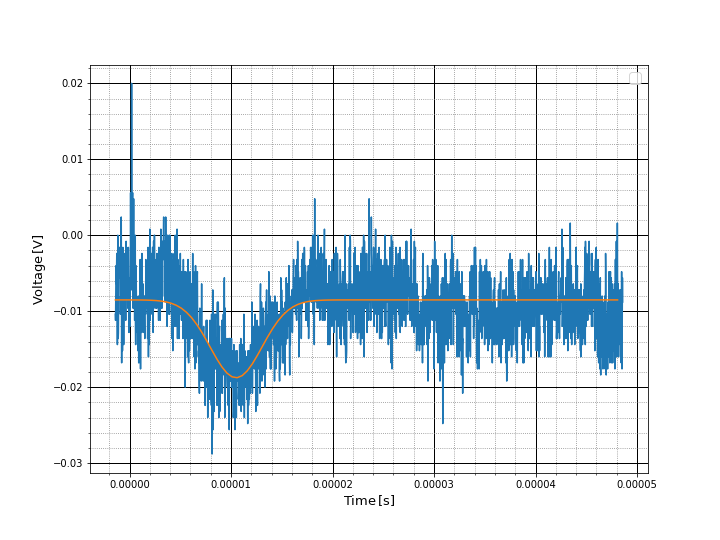
\includegraphics[scale=0.5]{Bild/A1}
	\centering
	\caption[Gaußfit an Messung bei Konst. Abstand]{Gaußfit an die Messungen der Elektronenwolken bei Konstantem Abstand von $3.6$\,mm und einer Spannung von $-36.0$\,V}
\end{figure}
\begin{figure}
	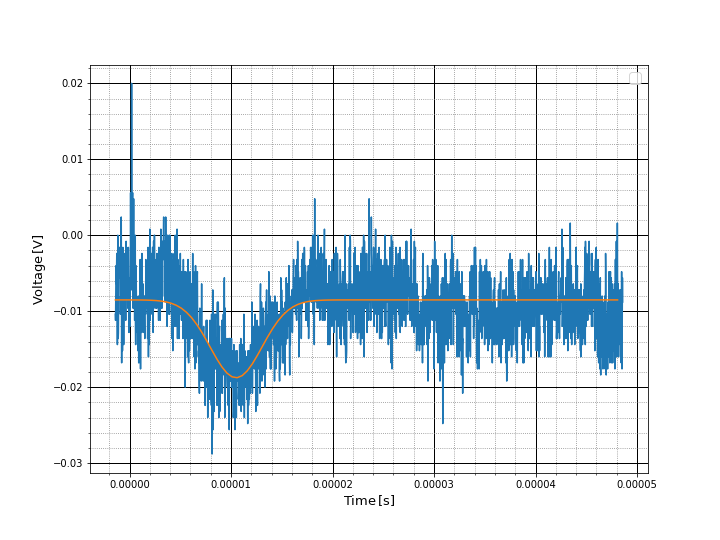
\includegraphics[scale=0.5]{Bild/A1}
	\centering
	\caption[Gaußfit an Messung bei Konst. Abstand]{Gaußfit an die Messungen der Elektronenwolken bei Konstantem Abstand von $3.6$\,mm und einer Spannung von $-40.0$\,V}
\end{figure}
\begin{figure}
	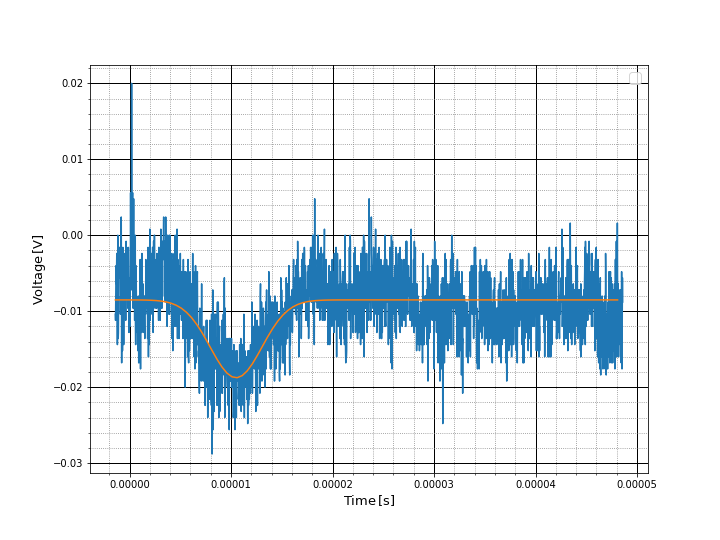
\includegraphics[scale=0.5]{Bild/A1}
	\centering
	\caption[Gaußfit an Messung bei Konst. Abstand]{Gaußfit an die Messungen der Elektronenwolken bei Konstantem Abstand von $3.6$\,mm und einer Spannung von $-44.0$\,V}
\end{figure}
\begin{figure}
	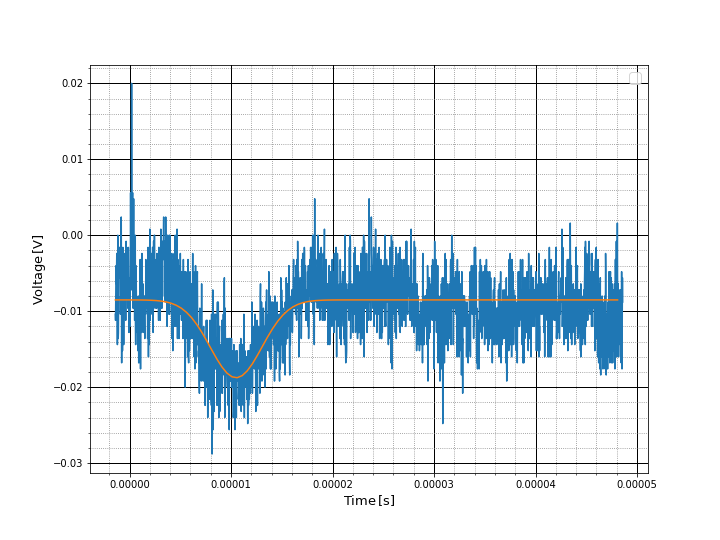
\includegraphics[scale=0.5]{Bild/A1}
	\centering
	\caption[Gaußfit an Messung bei Konst. Abstand]{Gaußfit an die Messungen der Elektronenwolken bei Konstantem Abstand von $3.6$\,mm und einer Spannung von $-46.0$\,V}
\end{figure}
\begin{figure}
	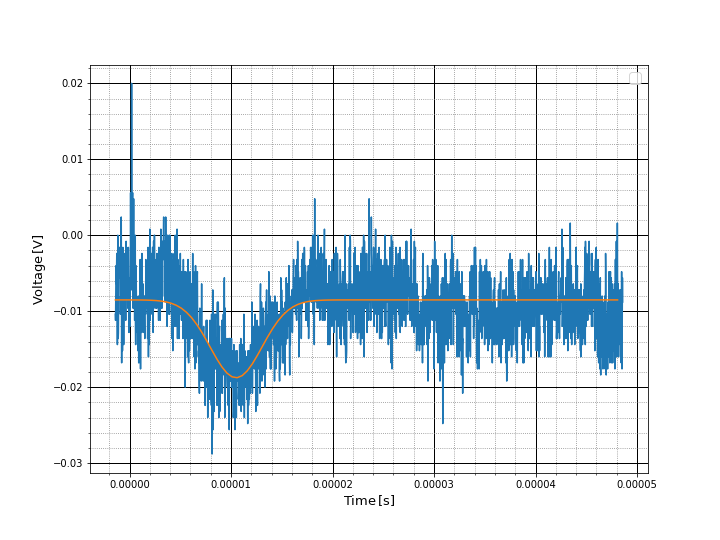
\includegraphics[scale=0.5]{Bild/A1}
	\centering
	\caption[Gaußfit an Messung bei Konst. Abstand]{Gaußfit an die Messungen der Elektronenwolken bei Konstantem Abstand von $3.6$\,mm und einer Spannung von $-48.0$\,V}
\end{figure}

%Lange Messungen

\begin{figure}[ht]
	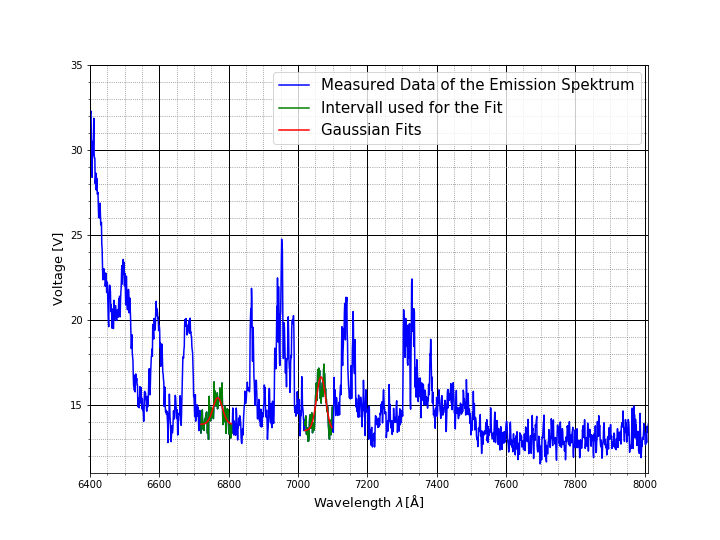
\includegraphics[scale=0.5]{Bild/ASg}
	\centering
	\caption{Gesamtes Spektrum von Americium mit Silizium aufgenommen.}
\end{figure}
\begin{figure}[ht]
	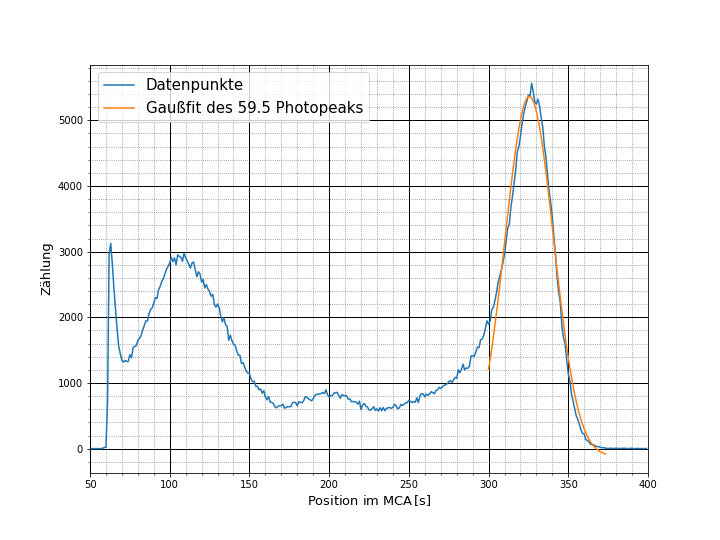
\includegraphics[scale=0.5]{Bild/ACg}
	\centering
	\caption{Gesamtes Spektrum von Americium mit CdTe aufgenommen.}
\end{figure}
\begin{figure}[ht]
	\includegraphics[scale=0.5]{Bild/CSg}
	\centering
	\caption{Gesamtes Spektrum von Cobalt mit Silizium aufgenommen.}
\end{figure}
\begin{figure}[ht]
	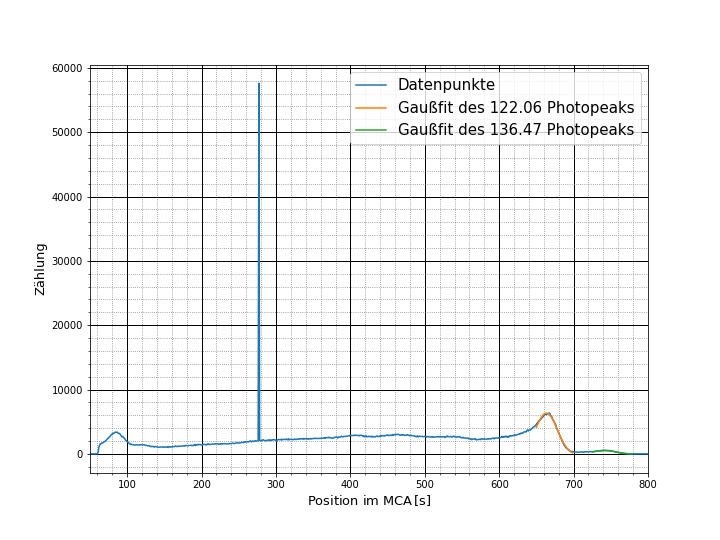
\includegraphics[scale=0.5]{Bild/CCg}
	\centering
	\caption{Gesamtes Spektrum von Cobalt mit CdTe aufgenommen.}
\end{figure}
\subsection{Laborbuch}
%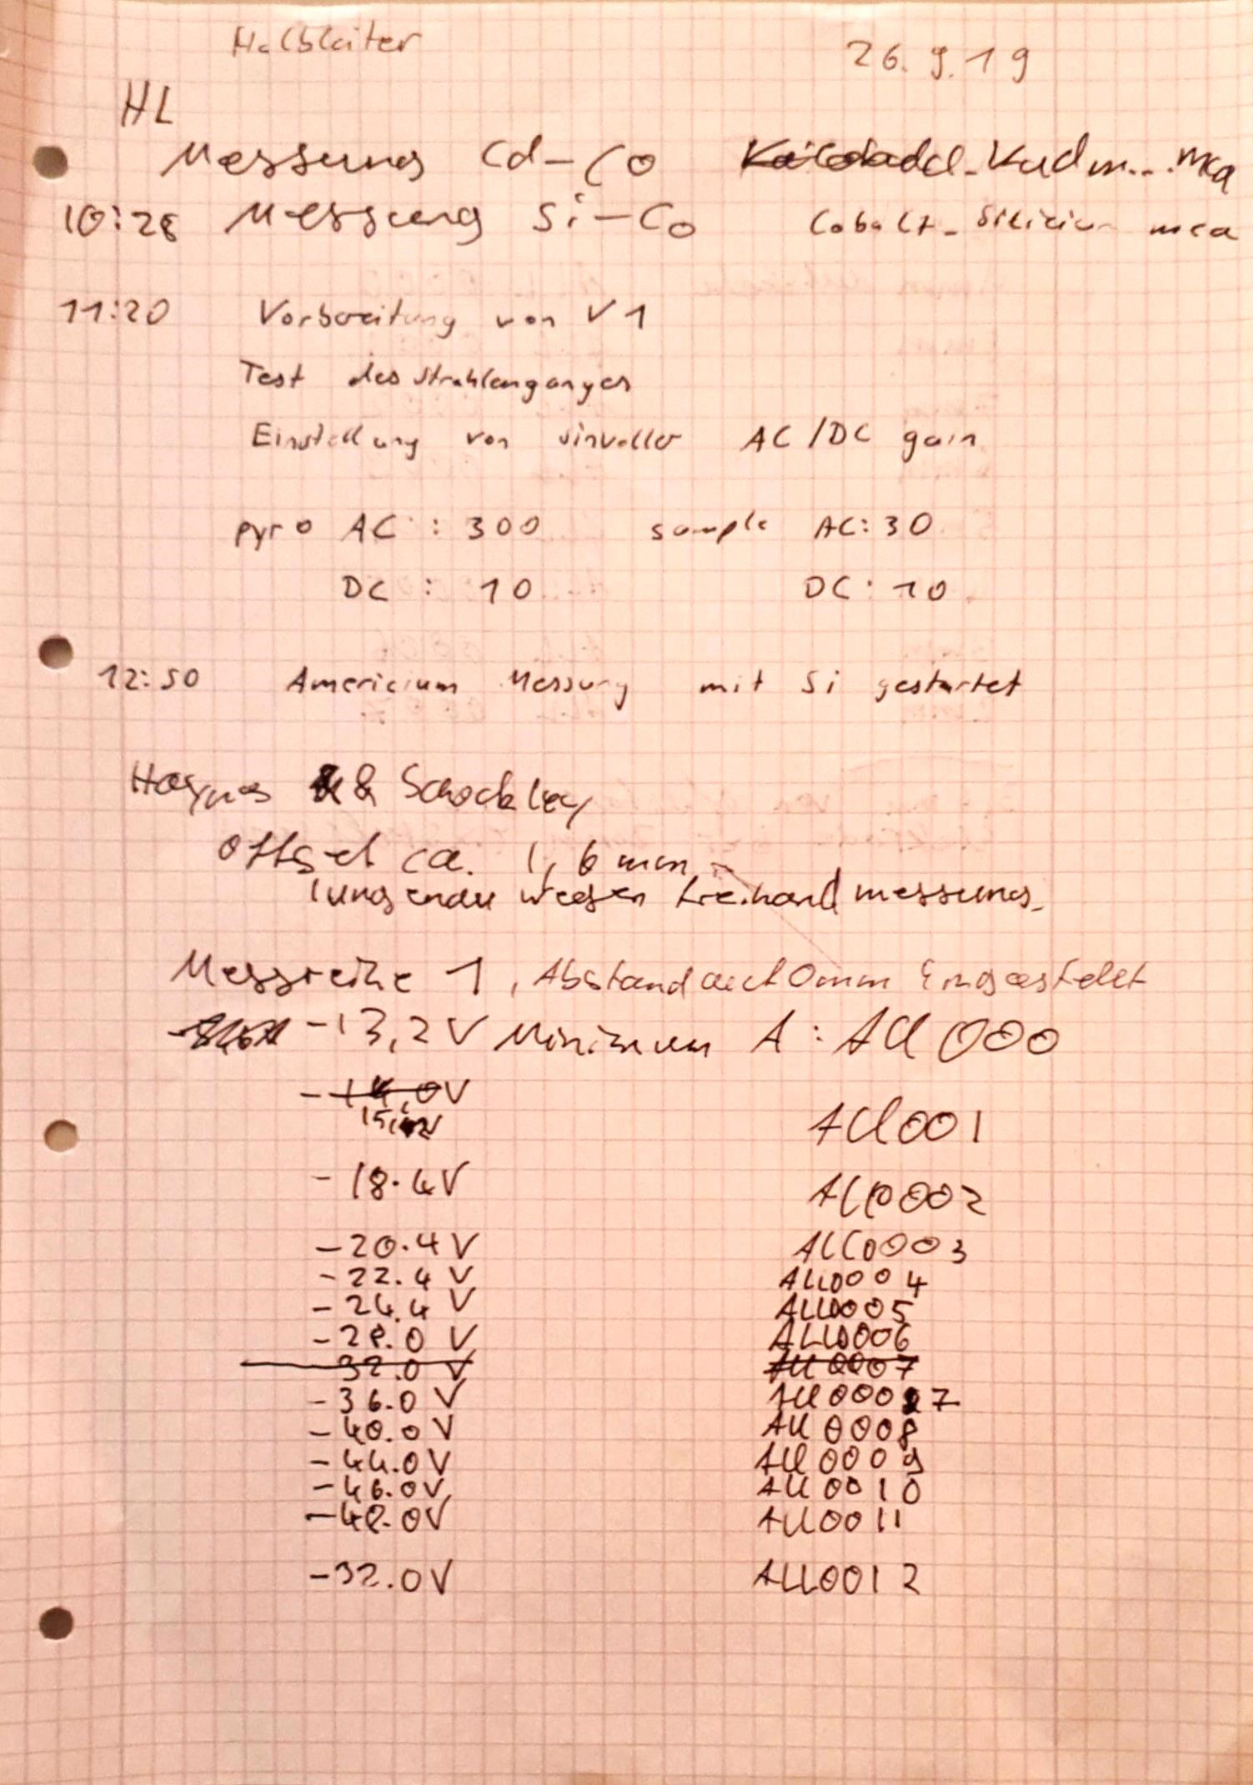
\includepdf[pages=-,scale=0.8]{Bilder/anhang/Halbleiter.pdf}
\end{document}